\documentclass[10pt,a4paper]{amsart}
\usepackage[margin=19mm]{geometry}
\usepackage{amsmath,amssymb,mathtools}
\usepackage[scr=rsfs,cal=euler]{mathalfa}
\usepackage{xfrac}
\usepackage[unicode,hidelinks,bookmarks=false]{hyperref}
\newcommand{\ie}{i.e.\ }
\newcommand{\cf}{cf.\ }
\newcommand{\resp}{respectively\ }
\newcommand{\Subsection}{\subsection}
\providecommand{\nobreakdash}{\nobreak\hbox{-}}
\setlength{\emergencystretch}{2em}
\multlinegap0pt
\usepackage{tikz}
\usepackage{amssymb}
\newtheorem{lemma}{Lemma}
\title{A Bijective Proof of an Unbalanced Wilf-Equivalence}
\author{Jensen Bridges, Michael Waite}
\date{Source: arXiv:2608.21684v1 (CC BY 4.0)}
\begin{document}
\maketitle

\noindent\emph{Source and licence.} A Bijective Proof of an Unbalanced Wilf-Equivalence. Version arXiv:2608.21684v1 (CC BY 4.0), distributed by arXiv under the Creative Commons Attribution 4.0 International licence, http://creativecommons.org/licenses/by/4.0/, as recorded in the arXiv licence metadata for this exact version and shown on the abstract page https://arxiv.org/abs/2608.21684v1. Full licence notice: \texttt{licenses/arxiv-2608.21684-CC-BY-4.0.txt}.\par\smallskip

\noindent\textit{Editorial scope.} Counted unit: the article's lemma lemma (source0.tex lines 133--142). The article's complete original proof of it is delivered with it (source0.tex lines 144--309, one \texttt{proof} environment of 166 lines). No mathematics is written, repaired or re-derived: the statement and the proof are the article's own lines, in the article's own notation, and no retained line is substituted or re-flowed.  No further source-local context is needed: every cross-reference of every retained line resolves inside the two delivered spans.  Nothing was omitted from any retained span, so the package carries no omission record.  No retained line contains a citation, so the wrapper carries no bibliography and no bibliography entry.  The retained lines contain the article's own diagram code, which the wrapper typesets with the standard tikz packages; no image file is delivered and the package declares no asset dependency.  Editorial formatting only, in addition: an AMS \texttt{amsart} preamble that restates the article's own declarations and macros used by the retained lines, namely the environments \texttt{lemma} on separate counters, together with the standard packages those lines need.  The retained environments print in this document as Lemma 1 in order of appearance, whereas the article prints the same items with the numbering of its own full document.  The complete native source of the article as distributed in the arXiv e-print for this exact version is bundled unchanged as \texttt{sources/208269/source0.tex}.
\begin{lemma}
    Let $p$ be a permutation avoiding $3412$, $45321$, and $54312$, and which is such that the rightmost $32$ entries participating in a $4321$ pattern are to the left of the leftmost $23$ entries participating in a $4231$. Then the following are true:
    \begin{enumerate}
        \item $\phi(p)$ avoids $3412$.
        \item $\phi(p)$ sends the leftmost entries participating as the $23$ in a $4231$ pattern to the rightmost entries participating as the $32$ in a $4321$ pattern.
        \item The leftmost $23$ entries in a $4231$ pattern in $\phi(p)$ are to the right of the leftmost $23$ entries in a $4231$ pattern in $p$.
        %\item $\phi(p)$ has no lexicographically left $4231$ of the lexicographically leftmost $4231$ in $p$.
        \item $\phi(p)$ avoids $45321$ and $54312$.
    \end{enumerate}
\end{lemma}

\begin{proof}
\begin{figure}[h]
        \centering
        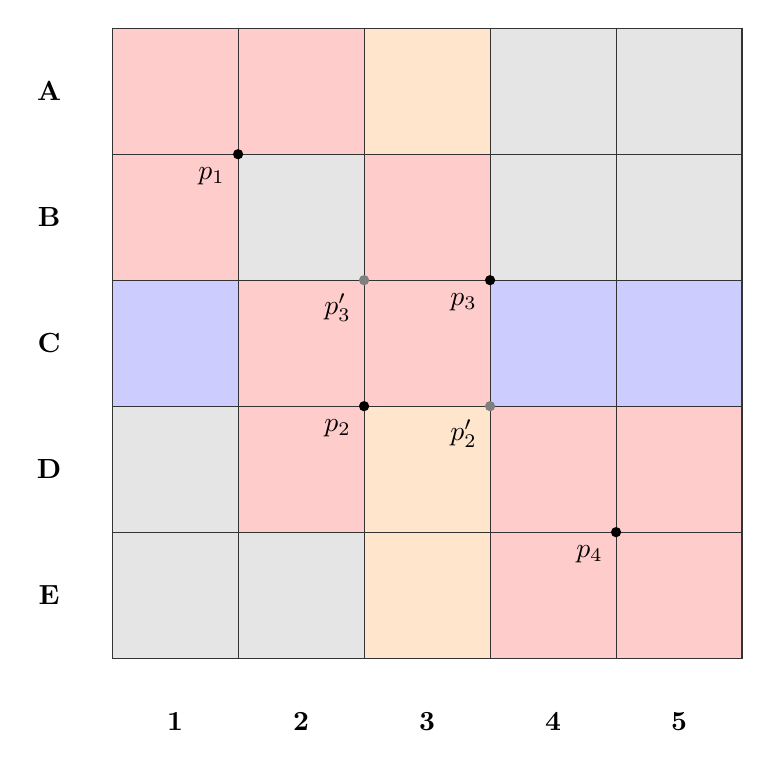
\begin{tikzpicture}[scale = 1.6, point/.style={circle,draw=black!100,fill=black!100,thick,
                     inner sep=0pt,minimum size=1mm},ghostpoint/.style={circle,draw=black!50,fill=black!50,thick,
                     inner sep=0pt,minimum size=1mm}
                          ]
                          
      \draw[draw = black!80!,fill=gray!20] (0,0) rectangle node[anchor= center]{} (1,1);
      \draw[draw = black!80!,fill=gray!20] (1,0) rectangle node[anchor= center]{} (2,1);
      \draw[draw = black!80!,fill=orange!20] (2,0) rectangle node[anchor= center]{} (3,1);
      \draw[draw = black!80!,fill=red!20] (3,0) rectangle node[anchor= center]{} (4,1);
      \draw[draw = black!80!,fill=red!20] (4,0) rectangle node[anchor= center]{} (5,1);

      \draw[draw = black!80!,fill=gray!20] (0,1) rectangle node[anchor= center]{} (1,2);
      \draw[draw = black!80!,fill=red!20] (1,1) rectangle node[anchor= center]{} (2,2);
      \draw[draw = black!80!,fill=orange!20] (2,1) rectangle node[anchor= center]{} (3,2);
      \draw[draw = black!80!,fill=red!20] (3,1) rectangle node[anchor= center]{} (4,2);
      \draw[draw = black!80!,fill=red!20] (4,1) rectangle node[anchor= center]{} (5,2);

      \draw[draw = black!80!,fill=blue!20] (0,1+1) rectangle node[anchor= center]{} (1,2+1);
      \draw[draw = black!80!,fill=red!20] (1,1+1) rectangle node[anchor= center]{} (2,2+1);
      \draw[draw = black!80!,fill=red!20] (2,1+1) rectangle node[anchor= center]{} (3,2+1);
      \draw[draw = black!80!,fill=blue!20] (3,1+1) rectangle node[anchor= center]{} (4,2+1);
      \draw[draw = black!80!,fill=blue!20] (4,1+1) rectangle node[anchor= center]{} (5,2+1);

      \draw[draw = black!80!,fill=red!20] (0,1+2) rectangle node[anchor= center]{} (1,2+2);
      \draw[draw = black!80!,fill=gray!20] (1,1+2) rectangle node[anchor= center]{} (2,2+2);
      \draw[draw = black!80!,fill=red!20] (2,1+2) rectangle node[anchor= center]{} (3,2+2);
      \draw[draw = black!80!,fill=gray!20] (3,1+2) rectangle node[anchor= center]{} (4,2+2);
      \draw[draw = black!80!,fill=gray!20] (4,1+2) rectangle node[anchor= center]{} (5,2+2);

      \draw[draw = black!80!,fill=red!20] (0,1+3) rectangle node[anchor= center]{} (1,2+3);
      \draw[draw = black!80!,fill=red!20] (1,1+3) rectangle node[anchor= center]{} (2,2+3);
      \draw[draw = black!80!,fill=orange!20] (2,1+3) rectangle node[anchor= center]{} (3,2+3);
      \draw[draw = black!80!,fill=gray!20] (3,1+3) rectangle node[anchor= center]{} (4,2+3);
      \draw[draw = black!80!,fill=gray!20] (4,1+3) rectangle node[anchor= center]{} (5,2+3);
      

      \node (pi) at (1,4) [point] [label=below left:$p_1$] {};
      \node (pj) at (2,2) [point] [label=below left:$p_2$] {};
      \node (pj) at (2,3) [ghostpoint] [label=below left:$p_3'$] {};
      \node (pi) at (3,3) [point] [label=below left:$p_3$] {};
      \node (pi) at (3,2) [ghostpoint] [label=below left:$p_2'$] {};
      \node (pj) at (4,1) [point] [label=below left:$p_4$] {};
      
      \node (E) at (-0.5,0.5) [] [label=center:\textbf{E}] {}; 
      \node (D) at (-0.5,1.5) [] [label=center:\textbf{D}] {};  
      \node (C) at (-0.5,2.5) [] [label=center:\textbf{C}] {};  
      \node (B) at (-0.5,3.5) [] [label=center:\textbf{B}] {};  
      \node (A) at (-0.5,4.5) [] [label=center:\textbf{A}] {};  

      \node (1) at (0.5,-0.5) [] [label=center:\textbf{1}] {}; 
      \node (2) at (1.5,-0.5) [] [label=center:\textbf{2}] {};  
      \node (3) at (2.5,-0.5) [] [label=center:\textbf{3}] {};  
      \node (4) at (3.5,-0.5) [] [label=center:\textbf{4}] {};  
      \node (5) at (4.5,-0.5) [] [label=center:\textbf{5}] {}; 

        \end{tikzpicture}
        \label{fig:placeholder}
    \end{figure}

    Let $p_1p_2p_3p_4$ be a $4231$ pattern in $p$ with entries chosen so that $p_2$ is the leftmost possible, then $p_3$ is the leftmost possible given this choice of $p_2$, then $p_1$ is the leftmost possible given this choice of $p_2$ and $p_3$, then $p_4$ is the leftmost possible given this choice of $p_1, p_2$, and $p_3$. The map $\phi$ will move $p_2$ to $p_2'$ and $p_3$ to $p_3'$. The red squares in the grid below indicate where there are no entries in $p$ due to the assumptions on $p$ above.

    Proof of 1:
    \\
    Suppose $\phi(p)$ did have a $3412$ pattern $q=q_1q_2q_3q_4$. This pattern must either include one of $p_2'$ and $p_3'$ and contain an entry in a blue box and an entry in an orange box, or it must contain both $p_2'$ and $p_3'$. This is because if $q$ has only one of $p_2'$ and $p_3'$ and has no entry in a blue box, then replacing that entry by $p_3$ or $p_2$ respectively would give a $3412$ pattern in $p$, which is a contradiction. Likewise if $q$ has only one of $p_2'$ and $p_3'$ and has no entry in an orange box, then replacing that entry by $p_2$ or $p_3$ respectively would give a $3412$ pattern in $p$, which is a contradiction.
    
    \begin{itemize}
        \item Case 1: Suppose first that the $3412$ pattern has only one of the shifted points. Suppose also that $q_1$ is in C1.
        \begin{itemize}
            \item If $p_3'$ is in the $3412$ pattern, then $p_3'$ must be $q_2$. Further, $q_3$ must be in D3 or E3 for an orange box to be included, and $q_4$ can be in D3, E3 (if $q_3$ is), C4, or C5. But this means that $q_1p_1q_3q_4$ is a $3412$ pattern in $p$ which is a contradiction. 
            \item If instead $p_2'$ is in the $3412$ pattern, then $p_2'$ must be either $q_3$ or $q_4$. If $p_2'$ is $q_3$, then $q_4$ must be in C4 or C5. In either case, $p$ then has a $3412$ pattern in $q_1p_1p_2q_4$. If $p_2'$ is instead $q_4$, then for an orange box to be occupied, $q_3$ must be in D3 or E3. If $q_3$ is in D3, then $p$ has a $45321$ pattern in $q_1p_1p_2q_3p_4$, and if $q_3$ is in E3, then $p$ has a $3412$ pattern in $q_1p_1q_3p_4$. 
        \end{itemize}
        \item Case 2: Suppose the $3412$ pattern again has only one of the shifted points but that $q_1$ is not in C1. 
        \begin{itemize}
            \item Suppose first $p_3'$ is in the pattern. In order for both an orange and a blue box to be occupied, we must have that $p_3'$ is $q_1$, $q_2$ is in A3, and $q_4$ must be in C4 or C5. However, if $q_4$ is in C4, then $p$ has a $45321$ pattern in $p_1q_2p_3q_4p_4$. If, on the other hand, $q_4$ is in C5, then $p$ has a $3412$ pattern in $p_1q_2p_4q_4$. 
            \item Now suppose $p_2'$ is in the pattern. Then because a blue box must be occupied and because an entry can only be below and to the right of $p_2'$ if it is in fact $p_4$, we must have that $p_2'$ is $q_3$ and $q_4$ is in C4 or C5. Further, for an orange box to be occupied, we must have that $q_2$ is in A3. If $q_4$ is in C4, then $p$ has a $45321$ pattern in $p_1q_2p_3q_4p_4$. If, on the other hand, $q_4$ is in C5, then $p$ has a $3412$ pattern in $p_1q_2p_4q_4$.
        \end{itemize}
        \item Case 3: Finally, suppose the $3412$ pattern contains both $p_2'$ and $p_3'$. We no longer require that both and orange and a blue box must be occupied by parts of the pattern $q_1q_2q_3q_4$. We split this into 4 cases depending on the parts of the pattern these points can act as.
        \begin{itemize}
            \item First, assume $p_3'$ is $q_1$ and $p_2'$ is $q_3$. Then $q_2$ must be in A3 and $q_4$ must be in C4 or C5.  If $q_4$ is in C4, then $p$ has a $45321$ pattern in $p_1q_2p_3q_4p_4$, and if $q_4$ is in C5, then $p$ has a $3412$ pattern in $p_1q_2p_4q_4$.
            \item Next, assume $p_3'$ is $q_1$ and $p_2'$ is $q_4$. Then $q_2$ must be in A3 and $q_3$ must be in D3 or E3. In either case, $p$ has a $3412$ pattern in $p_1q_2q_3p_3$.
            \item Now, assume $p_3'$ is $q_2$ and $p_2'$ is $q_3$. Then $q_1$ must be in C1 and $q_4$ must be in C4 or C5. In either case, $p$ then has a 3412 pattern in $q_1p_1p_2q_4$.
            \item Finally, assume $p_3'$ is $q_2$ and $p_2'$ is $q_4$. Then $q_1$ must be in C1 and $q_3$ must be in D3 or E3. If $q_3$ is in E3, then $p$ has a $3412$ pattern in $q_1p_1q_3p_4$, and if $q_3$ is in D3, then $p$ has a $45321$ pattern in $q_1p_1p_2q_3p_4$. 
        \end{itemize}
    \end{itemize}  

    \vspace{10pt}

    
    Proof of 2:
    \\
    Suppose $\phi(p)$ does have a $4321$ pattern $q=q_1q_2q_3q_4$ in which $q_2q_3$ is to the right of $p_3'p_2'$. Again, either $p_2'$ and $p_3'$ are in $q$, or exactly one of $p_2'$ and $p_3'$ is in $q$ and $q$ must contain an entry in a blue box and an entry in an orange box. 

    \begin{itemize}
        \item Case 1: Suppose first only one of the points $p_2'$, $p_3'$ is in $q$.
        \begin{itemize}
            \item Then because $q$ must be entirely decreasing, there is no way for $q$ to have an entry in an orange box and in a blue box. 
        \end{itemize}
        
        \item Case 2: Suppose both of $p_3'$ and $p_2'$ are in $q$. 
        \begin{itemize}
            \item Since there are no entries allowed in C3, then $p_3'$ and $p_2'$ must be consecutive entries of $q$. Further, since $q_2q_3$ is to the right of $p_3'p_2'$, then $p_3'$ and $p_2'$ must be $q_1$ and $q_2$. But there is only one point which can go below and to the right of $p_2'$, namely $p_4$, so there is no valid way to place $q_3$ and $q_4$, so we have a contradiction. 
        \end{itemize}
        
    \end{itemize}
     

    \vspace{10pt}
    
    Proof of 3: Suppose there is a $4231$ pattern $q=q_1q_2q_3q_4$ in $\phi(p)$ with $q_2q_3$ to the left of $p_2p_3$.
    \begin{itemize}
        \item Case 1: Suppose only one of $p_2'$ and $p_3'$ are in $q$. Then it must be the case that $q$ has an entry in C1 and an entry in A3 or both an entry in D3 or $E3$ and an entry in C4 or C5, as otherwise $\phi(p)$ will have a $3412$ pattern which is forbidden by $(1)$.
        \begin{itemize}
            \item In the former case, then $q_2$ must be in C1 and $q_3$ must be in A3 since $4231$ only has an increase in those positions, but then there is nowhere to place $q_1$ so this is a contradiction. 
            \item In the latter case, then $q_2$ must be in D3 or E3 and $q_3$ must be in C4 or C5. But then $q_2q_3$ is to the right of $p_2p_3$, which contradicts the assumption.
        \end{itemize}
        \item Case 2: If both $p_2'$ and $p_3'$ are in $q$, then in order for $q_2q_3$ to be to the left of $p_2p_3$, $p_3'$ must be $q_2$ or $q_3$. 
        \begin{itemize}
            \item If $p_3'$ is $q_2$, then $q_3$ must go in A3 and there is nowhere to place $q_1$.
            \item If $p_3'$ is $q_3$, then $q_2$ must go in C1 and again there is nowhere to place $q_1$.
        \end{itemize}
    \end{itemize}


    \vspace{10pt}
    
    Proof of 4:
    \\
    Suppose $\phi(p)$ did have a $45321$ pattern $q_1q_2q_3q_4q_5$. This pattern must include one of either $p_2'$ or $p_3'$, and must contain an entry in a blue box and an entry in an orange box, or it must contain both $p_2'$ and $p_3'$.

    \begin{itemize}
        \item Case 1: Suppose first that $q_1$ is in C1. By (1), there can be no entries in D3 or E3 since otherwise $\phi(p)$ would have a $3412$ pattern with $q_1$, $p_1$, this point, and $p_2'$.
        \begin{itemize}
            \item If $p_3'$ is in the pattern, then no orange box can be occupied. 
            \item If instead $p_2'$ is in the pattern, then it must act as $q_5$ with $q_2, q_3,q_4$ in C1 since $q_1$ is. Again, then no orange box can be occupied. 
        \end{itemize}
        \item Case 2: Suppose that the pattern still has exactly one of the shifted points but assume instead that $q_1$ is not in C1. 
        \begin{itemize}
            \item Suppose first that $p_3'$ is part of the $45321$ pattern. Then in order for both orange and blue boxes to contain pieces of the $45321$ pattern, $p_3'$ must be $q_1$. Further, A3 must contain $q_2$ and the blue boxes must contain $q_3,q_4,q_5$. But then replacing $p_3'$ by $p_1$ gives a $45321$ pattern in $p$, a contradiction.
            \item Now suppose instead that $p_2'$ is part of the $45321$ pattern. Then $p_2'$ must be $q_5$, and $q_1,q_2,q_3,q_4$ must be in B2 and/or A3. Thus, there are no parts of the pattern in a blue box, a contradiction. 
        \end{itemize}
        \item Case 3: Finally, assume both $p_2'$ and $p_3'$ are in the $45321$ pattern. Because no entries are allowed in C3 or anywhere below and to the right of $p_2'$ (except $p_4$), these points must act as $q_3$ and $q_4$ with $p_4$ as $q_5$, or $q_4$ and $q_5$.
        \begin{itemize}
            \item If $p_3'$ and $p_2'$ are $q_3$ and $q_4$ with $p_4$ as $q_5$, then $q_1$ and $q_2$ must both be in B2. Then $p$ has a $3412$ pattern in $q_1q_2p_2p_3$.
            \item If instead these points act as $q_4$ and $q_5$, then $q_1, q_2, q_3$ must all be in B2 and we have the same issue as above. 
        \end{itemize}
    \end{itemize}
    

    Now, suppose $\phi(p)$ has a $54312$ pattern $q_1q_2q_3q_4q_5$. Again, this pattern must contain one of $q_2'$ and $q_3'$ and an entry in an orange and a blue box, or both of the shifted points. 

    \begin{itemize}
        \item Case 1: Suppose first that $q_1$ is in C1 and exactly one of the shifted points is included. Then again because of (1), we can't have any entries in D3 or E3. Also, $p_3'$ can't be in the pattern, so $p_2'$ must be. Further, it must be $q_5$, otherwise there are no pieces in an orange box, and C1 must have $q_1,q_2,q_3$ in a 321 pattern. However, since D3 and E3 are blocked, there's nowhere to place $q_4$. 
        \item Case 2: Now suppose $q_1$ is not in C1 but we still have exactly one of the shifted points included.
        \begin{itemize}
            \item Suppose first $p_3'$ is in the $54312$ pattern. For a blue box to be populated by the pattern, $p_3'$ must be $q_3$. Then $p$ has a $54312$ pattern in $p_1q_1q_2q_4q_5$, a contradiction. 
            \item If instead $p_2'$ is in the pattern, then for a blue box to be populated, $p_2'$ must be $q_4$, with $q_1q_2q_3$ in B2 or A3 and $q_5$ in C4 or C5. In order for an orange box to be populated, it must be true that $q_1q_2q_3$ is in A3. If $q_5$ is in C4, then $p_1q_1p_3q_5p_4$ forms a $45321$ pattern in $p$, and if $q_5$ is in C5 then $q_1q_2q_3p_4q_5$ forms a $54312$ pattern in $p$. 
        \end{itemize}
        \item Case 3: Finally, suppose both $p_2'$ and $p_3'$ are in the $54312$ pattern. Then $p_3'$ must be $q_3$ and $p_2'$ can be $q_4$ or $q_5$. In both cases, $q_1$ and $q_2$ must be in B2 in a 21 pattern. Then $p$ has a $54312$ pattern in $p_1q_1q_2p_2p_3$.
    \end{itemize}

     

\end{proof}

\end{document}
